
\subsection{{\idletime}が一般の場合}
\label{subsec:LineDifferentTimelimit}

全点の{\idletime}が等しい場合は
どの頂点も高々1人の巡査が担当するため
単純になっていたが,
{\idletime}が一般の場合は,
頂点を複数の巡査が交代で訪問して警備する必要がある場合が存在する.
%
図\ref{tikz:multiAgentExample2}(左)の例では,
中央の{\idletime}の短い2つの頂点を
2人の巡査が交互に訪問しており,
また,全点の{\idletime}が等しい場合と異なり
各巡査の最適な運行はなんらかの区間の往復であるとは限らないことも分かる.


また,
この例では左の巡査は左端の点を{\idletime}$10$ちょうどごとに訪問しているが,
左端の点の{\idletime}から順に巡査の運行を決定することも難しい次のような例が存在する.
図\ref{tikz:multiAgentExample2}(中央)の例では
{\idletime}$8$の左端の点をあえてより短い$6$ごとに訪問することで全点を警邏できるが,
同じグラフについて,
図\ref{tikz:multiAgentExample2}(右)のように左の巡査が
左端の点の{\idletime}ぎりぎりの時間まで右の方へ動き頂点をなるべく多くの時間訪問して左端へ帰る運行を選ぶと
右の巡査がどのような動き方をしても{\idletime}を超え警備できない頂点が生まれてしまう.



\begin{figure}[h]
  \centering
  \begin{tabular}{ccc}

  \begin{minipage}{0.32\hsize}
    \centering
    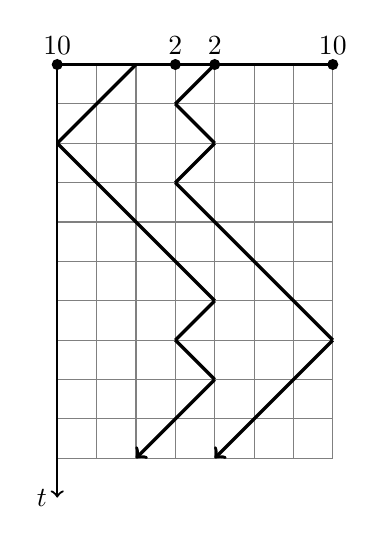
\begin{tikzpicture}
      \draw [help lines,thin,step=5mm] (0,-5.0) grid (3.5,0);
      \draw[thick] (0,0) -- (3.5,0) node [below] {};
      \draw[thick, ->] (0,0) -- (0,-5.5) node [left] {$t$};

      \fill ( 0   , 0) coordinate (c1) circle (2pt) node [above] {10};
      \fill ( 1.5 , 0) coordinate (c2) circle (2pt) node [above] {2};
      \fill ( 2.0 , 0) coordinate (c3) circle (2pt) node [above] {2};
      \fill ( 3.5 , 0) coordinate (c5) circle (2pt) node [above] {10};

      \draw[very thick,- ] ( 1.0, 0  )--(   0,-1.0);
      \draw[very thick,- ] (   0,-1.0)--( 2.0,-3.0);
      \draw[very thick,- ] ( 2.0,-3.0)--( 1.5,-3.5);
      \draw[very thick,- ] ( 1.5,-3.5)--( 2.0,-4.0);
      \draw[very thick,->] ( 2.0,-4.0)--( 1.0,-5.0);

      \draw[very thick,- ] ( 2.0, 0  )--( 1.5,-0.5);
      \draw[very thick,- ] ( 1.5,-0.5)--( 2.0,-1.0);
      \draw[very thick,- ] ( 2.0,-1.0)--( 1.5,-1.5);
      \draw[very thick,- ] ( 1.5,-1.5)--( 3.5,-3.5);
      \draw[very thick,->] ( 3.5,-3.5)--( 2.0,-5.0);
    \end{tikzpicture}
  \end{minipage}

  \begin{minipage}{0.32\hsize}
    \centering
    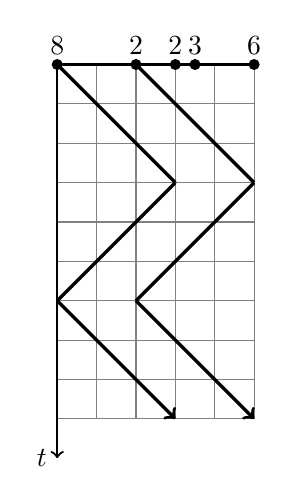
\begin{tikzpicture}
      \draw [help lines,thin,step=5mm] (0,-4.5) grid (2.5,0);
      \draw[thick] (0,0) -- (2.5,0) node [below] {};
      \draw[thick, ->] (0,0) -- (0,-5) node [left] {$t$};

      \fill ( 0   , 0) coordinate (c1) circle (2pt) node [above] {8};
      \fill ( 1   , 0) coordinate (c2) circle (2pt) node [above] {2};
      \fill ( 1.5 , 0) coordinate (c3) circle (2pt) node [above] {2};
      \fill ( 1.75, 0) coordinate (c4) circle (2pt) node [above] {3};
      \fill ( 2.5 , 0) coordinate (c5) circle (2pt) node [above] {6};

      % \draw[very thick,red,<->] (1.75,-0.75)--(1.75,-2.25);

      \draw[very thick,- ] ( 0  , 0  )--( 1.5,-1.5);
      \draw[very thick,- ] ( 1.5,-1.5)--( 0  ,-3  );
      \draw[very thick,->] ( 0  ,-3  )--( 1.5,-4.5);
      \draw[very thick,- ] ( 1  , 0  )--( 2.5,-1.5);
      \draw[very thick,- ] ( 2.5,-1.5)--( 1  ,-3  );
      \draw[very thick,->] ( 1  ,-3  )--( 2.5,-4.5);
    \end{tikzpicture}
  \end{minipage}

  \begin{minipage}{0.32\hsize}
    \centering
    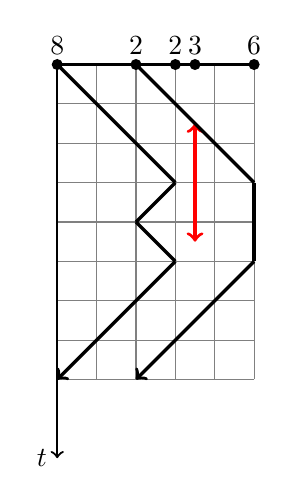
\begin{tikzpicture}
      \draw [help lines,thin,step=5mm] (0,-4) grid (2.5,0);
      \draw[thick] (0,0) -- (2.5,0) node [below] {};
      \draw[thick, ->] (0,0) -- (0,-5) node [left] {$t$};

      \fill ( 0   , 0) coordinate (c1) circle (2pt) node [above] {8};
      \fill ( 1   , 0) coordinate (c2) circle (2pt) node [above] {2};
      \fill ( 1.5 , 0) coordinate (c3) circle (2pt) node [above] {2};
      \fill ( 1.75, 0) coordinate (c4) circle (2pt) node [above] {3};
      \fill ( 2.5 , 0) coordinate (c5) circle (2pt) node [above] {6};

      \draw[very thick,red,<->] (1.75,-0.75)--(1.75,-2.25);

      \draw[very thick,- ] ( 0  , 0  )--( 1.5,-1.5);
      \draw[very thick,- ] ( 1.5,-1.5)--( 1  ,-2  );
      \draw[very thick,- ] ( 1  ,-2  )--( 1.5,-2.5);
      \draw[very thick,->] ( 1.5,-2.5)--( 0  ,-4  );

      \draw[very thick,- ] ( 1  , 0  )--( 2.5,-1.5);
      \draw[very thick,- ] ( 2.5,-1.5)--( 2.5,-2.5);
      \draw[very thick,->] ( 2.5,-2.5)--( 1  ,-4  );
    \end{tikzpicture}
  \end{minipage}

  \end{tabular}
  \caption{巡査の協力が必要な例.
    横軸を頂点の座標,縦軸を時刻として巡査の軌跡を表す.
    点の上の数値は{\idletime}を表す.
    \label{tikz:multiAgentExample2}}
\end{figure}




これらの例は,協力が発生する場合巡査の運行を個別に決定するのは難しいということを示唆している.
しかしながら,この{\idletime}が一般の場合での{\graphLine}上の{\patProb}の困難性を示すこともできなかった.
そこで,{\idletime}より短い間隔で点を訪問しうることで運行の決定を複雑になる例が存在したことを踏まえて,
1章で定義した{\timeSpecifiedPatProbDecision}を考える.




\begin{defi}
  $X \subset \Zset \times \Nset$とする.
  任意の$(t_1, x_1), (t_2, x_2) \in X$が
  $\abs{x_1 - x_2} \leq \abs{t_1 - t_2}$
  を満たすとき,$X$は運行可能であるという.
\end{defi}


任意の運行可能な集合$X$に対して,
{\graphLine}上の巡査の運行$a$であって,
$X$のすべての元$(t, x)$に対して$a(t) = x$を満たすものが存在することは簡単に示すことができる.
これにより,
グラフが{\graphLine}の場合の{\timeSpecifiedPatProbDecision}は次のようにも記述できる.

\begin{timeSpecifiedProblemOnLine}
  正の整数$m$(巡査の人数を表す)
  と自然数の組$(q_i, r_i, x_i)_{ i \in \{ 1, \ldots, n \} }$が与えられる.
  集合
  $\{ (q_i k + r_i, x_i) \mid i \in \{1, \ldots, n\}, k \in \Zset \}$
  を$m$個以下の運行可能な集合に分割できるか判定せよ.
\end{timeSpecifiedProblemOnLine}


% これを解くために次の副問題を考える.

% 1周期分だけ取り出して周期的分割可能であることと元のXが分割可能であることが一致することを説明し
% アルゴリズムでは無限集合の周期的な分割を与えてYesかNoを答える
この問題では,
$X := \{ (q_i k + r_i, x_i) \mid i \in \{1, \ldots, n\}, k \in \Zset \}$
という無限集合の分割が可能か判定しなければならないが,
実際には$X$の点は時刻(組$(t, x) \in X$の第1要素)について周期的であるため,
1周期分の有限部分集合を以下に定義する「周期的に運行可能な」集合に分割できるかどうかさえ
判定すればよい.

\red{理由を説明}



\begin{defi}
  $T$を正の整数,$X \subset \Zset \times \Nset$を有限集合とする.
  任意の$(t_1, x_1), (t_2, x_2) \in X$が
  $\abs{x_1 - x_2} \leq \abs{t_1 - t_2}$
  かつ
  $\abs{x_1 - x_2} \leq \abs{T + t_1 - t_2}$
  を満たすとき,$X$は周期$T$で運行可能であるという.
\end{defi}



\begin{greedyAlgorithmForTimeSpecifiedProblemOnLine}
  入力を$(m, (q_i, r_i, x_i)_{ i \in \{ 1, \ldots, n \} })$とする.
  始めに
  $T := lcm(q_1, \ldots, q_n)$,
  $X := \{ (q_i k + r_i, x_i) \mid i \in \{1, \ldots, n\}, k \in \Zset \}$,
  $L((\alpha, \beta)) := \{(t, x) \mid x - \beta \leq \abs{t - \alpha} \}$と記号を定義する.

  まず$X$の部分集合$S := \{ (x, t) \in X \mid -T \leq t < 2T \}$を求める.
  初期値を$\mathcal{B} = \{\}$, $B_0 = S$, $B' = S$, $i = 0$とし,
  $B_i \neq \emptyset$である限り1.から4.を繰り返す.
  \begin{enumerate}
    \item $i \gets i + 1$, 
    \item $B_i \gets B' \cap \left( \bigcap_{p \in B'} L(p) \right)$, 
    \item $B' \gets B' \setminus B_i$, 
    \item $\mathcal{B} \gets \mathcal{B} \cup \{ B_i \}$.
  \end{enumerate}

  $\card{\mathcal{B}} > m$ならば「分割不可能」と答え,
  そうでないときは「分割可能」と答え終了する.
  % そうでないときは分割可能と答えたうえで,
  % $\mathcal{B}$の各元を時刻方向に$[0, T)$に制限したもの
  % $\mathcal{C} := \{ \{ (t, x) \in B \mid 0 \leq t < T \} \mid B \in \mathcal{B} \}$
  % を出力して終了する.
\end{greedyAlgorithmForTimeSpecifiedProblemOnLine}

% 副問題は主問題の判定を行いさらに繰り返し運行可能分割を求める問題なので,
% 主問題の判定ができていることをここで説明する必要がある.
この{\timeSpecifiedPatProbOnLineAlg}が
\begin{itemize}
  \item 「分割不可能」と答えるとき,
    $X$も$m$個の運行可能な集合に分割することはできない.
    実際,
    $X$が$m$個の運行可能な集合に分割できるとき,
    $S := \{ (t, x) \in X \mid -T \leq t < 2T \}$
    は$X$の部分集合であるから$m$個の運行可能な集合に分割できるが,
    その場合は{\timeSpecifiedPatProbOnLineAlg}は必ず$m$個の運行可能な集合への分割を答える.
    これは次の理由による.
    {\graphLine}においては順序保存運行の存在と同様に,
    $S$が$m$個の運行可能な集合へ分割可能ならば
    $S$の$m$個の運行可能な集合への分割であって順序保存なものが存在する.
    ここで,分割$\mathcal{B'} = \{ B'_1, \ldots, B'_m \}$が順序保存であるとは,
    対応する運行$(b_1, \ldots, b_m)$が順序保存運行になることである.
    {\timeSpecifiedPatProbOnLineAlg}中で得られる$S$の分割$\mathcal{B} = \{ B_1, \ldots, B_m \}$は
    任意の順序保存な$S$の分割を選び$\mathcal{B'} = \{ B'_1, \ldots, B'_m \}$と整数$k$に対し,
    $\bigcup_{1 \leq i \leq k} B'_i \subseteq \bigcup_{1 \leq i \leq k} B_i$
    を満たしており,これにより
    $S$が$m$個の運行可能な集合へ分割可能ならば
    {\timeSpecifiedPatProbOnLineAlg}は必ず$m$個の運行可能な集合への分割を答えることが分かる.
  \item 「分割可能」と答えるとき,
    $X$も$m$個の運行可能な集合に分割することができる.
    実際,
    分割可能と答えるときには分割$\mathcal{C}$を出力するが,
    $\mathcal{C}$の各元$C$は
    周期$T$で繰り返し運行可能な集合である.
    これは,途中の各$B \in \mathcal{B}$が$L$の定義から運行可能集合となっており,
    $B$の$[-T, 2T)$の範囲が運行可能であれば$[0, T)$の範囲は
    定義から周期$T$で繰り返し運行可能となるためである.

    集合
    $X := \{ (q_i k + r_i, x_i) \mid i \in \{1, \ldots, n\}, k \in \Zset \}$
    の分割$\mathcal{A} = \{ A_1, \ldots, A_m \}$は次のように構成すればよい.
    $k \in \Zset$に対して,$X$の部分集合
    $\{ (t, x) \in X \mid kT \leq t < (k + 1)T \}$
    を$\mathcal{C}$の分割の仕方で分割したものを$\{ C_{k1}, \ldots, C_{km} \}$とする.
    $A_i := \bigcup_{k \in \Zset} C_{ki}$と定義すると,
    $C_{ki}$が周期$T$で繰り返し運行可能な集合であるから,
    $A_i$は運行可能な集合となる.
    % $\mathcal{A}$は$X$を$m$個の運行可能な集合へ分割したものとなっている.
\end{itemize}
以上より,{\timeSpecifiedPatProbOnLineAlg}は副問題を解く.
